\section{Exceptions, Errors}
Errors:
\begin{itemize}
    \itemsep0em
    \item Schwerwiegende Fehler, \textbf{nicht behandeln!}
    \item Fehler in JVM: OutOfMemoryError, ...
    \item Programmierfehler: AssertionError
\end{itemize}
Exceptions:
\begin{itemize}
    \itemsep0em
    \item Laufzeitfehler, die \textbf{behandelbar} sind
    \item fehlerhafte Bedienung, Parameter, ...
    \item siehe auch Checked / Unchecked \ref{checked,unchecked}
\end{itemize}
% Exceptions (Ausnahmen) dienen als Mittel zur kontrollierten Reaktion von Laufzeitfehlern, 
% z.B. bei logischen Programmfehlern, fehlerhafter Bedienung oder Probleme der JVM.

\subsubsection{Checked, Unchecked}\label{checked,unchecked}
Checked:
\begin{itemize}
    \itemsep0em
    \item Exception muss behandelt werden ODER
    \item \verb|throws|-Deklaration im Methodenkopf
    \item Wird vom Compiler geprüft
\end{itemize}

Unchecked:
\begin{itemize}
    \itemsep0em
    \item Kein \verb|throws| oder Behandlung nötig
    \item \verb|RuntimeException| und Error, sowie ihre Unterklassen
    \item Wird nicht vom Compiler geprüft
\end{itemize}

\subsection{Exception auslösen}
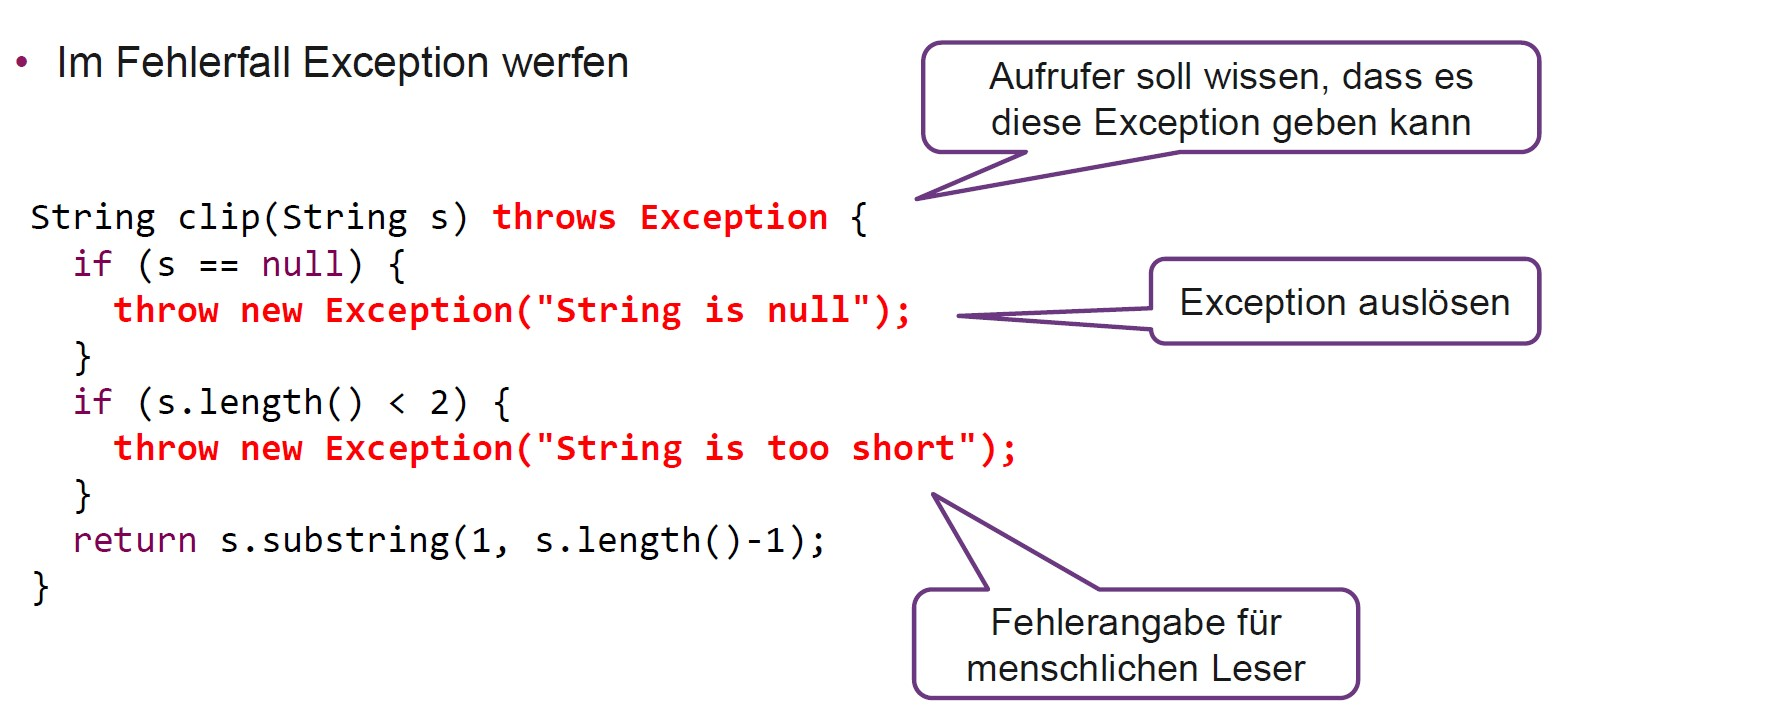
\includegraphics[width=\linewidth]{pictures/exception-throw.jpg}

\subsubsection{throws-Deklaration}
Die Methode muss alle potentiellen Exceptions deklarieren, die der Aufrufer erhalten könnte. (Ausser) %TODO: Unchecked Exceptions

Der Aufrufer muss die Exception behandeln (fangen) oder weiterreichen.

\subsection{Exception behandeln}
\begin{minipage}{0.6\columnwidth}
    \begin{itemize}
        \itemsep0em
        \item Regulärer Code (\verb|try-Block|)
        \item Fehlerbehandlung (\verb|catch|-Block)
        \begin{itemize}
            \itemsep0em
            \item Exception im \verb|try-Block| $\rightarrow$ \verb|catch|-Block
            \item Keine Exception: \verb|catch|-Block wird nicht ausgeführt
        \end{itemize}
        \item Opt. \verb|finally|-Block: Wird immer durchlaufen
    \end{itemize}
\end{minipage}
\hfill
\begin{minipage}{0.35\columnwidth}
    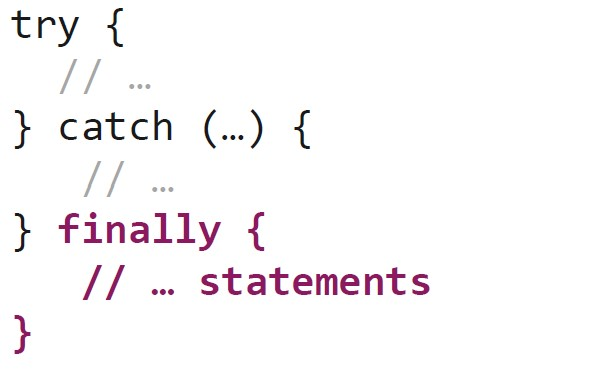
\includegraphics[width=\linewidth]{pictures/try-catch-finally.jpg}
\end{minipage}

Bei mehreren \verb|catch|-Blöcken wird \textbf{nur} der erste Passende (von oben nach unten gesucht) ausgeführt. 

Falls Exception nicht behandelt wird, wird die Exception zum nächsthöheren Aufrufer geschickt. 
Wenn dies \verb|main()| ist, wird die Exception an die JVM geworfen und das Programm abgebrochen.

\subsubsection{try-with-resources}
Für Objekte, die geschlossen werden müssen (Interface \verb|AutoCloseable|)\\
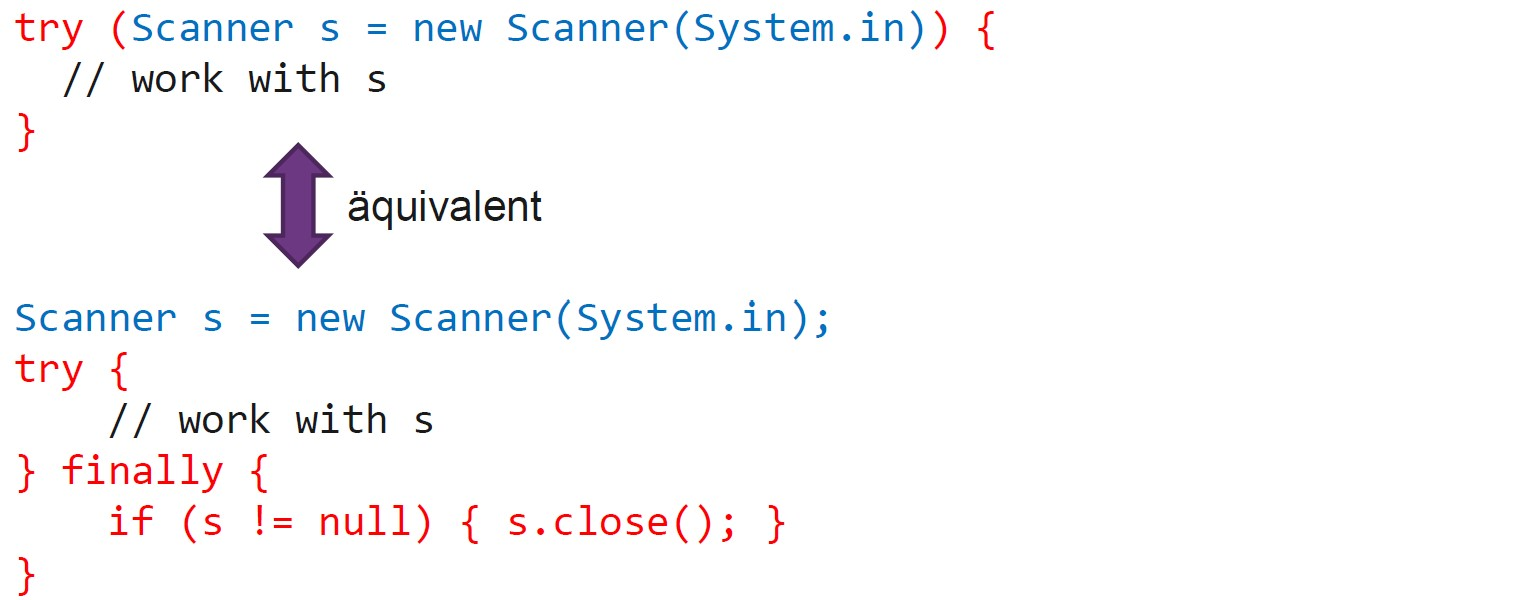
\includegraphics[width=\linewidth]{pictures/try-with-resources.jpg}
